%**************************************************************************************
% License:
% CC BY-NC-SA 4.0 (http://creativecommons.org/licenses/by-nc-sa/4.0/)
%**************************************************************************************

\documentclass[notes]{beamer}

\mode<presentation> {

\usetheme{Madrid}

% Burnt orange
\definecolor{burntorange}{rgb}{0.8, 0.33, 0.0}
\colorlet{beamer@blendedblue}{burntorange}
% Pale yellow
\definecolor{paleyellow}{rgb}{1.0, 1.0, 0.953}
\setbeamercolor{background canvas}{bg=paleyellow}
% Secondary and tertiary palett
\setbeamercolor*{palette secondary}{use=structure,fg=white,bg=burntorange!80!black}
\setbeamercolor*{palette tertiary}{use=structure,fg=white,bg=burntorange!60!black}

% To remove the footer line in all slides uncomment this line
%\setbeamertemplate{footline}
% To replace the footer line in all slides with a simple slide count uncomment this line
%\setbeamertemplate{footline}[page number]

% To remove the navigation symbols from the bottom of all slides uncomment this line
%\setbeamertemplate{navigation symbols}{}
}

\usepackage{amsmath}
\usepackage{bm}
\usepackage{breqn}
\usepackage{cancel}
\usepackage{graphicx} % for figures
\usepackage{subcaption} % for subplots 
\usepackage[labelsep=space,tableposition=top]{caption}
\renewcommand{\figurename}{Fig.} 
\usepackage{cleveref}
\usepackage{caption,subcaption}% http://ctan.org/pkg/{caption,subcaption}
\usepackage{booktabs} % Allows the use of \toprule, \midrule and \bottomrule in tables
\usepackage{multirow}
\usepackage{tabularx}
\usepackage{siunitx}
\usepackage{cleveref}
\usepackage{xcolor}
\usepackage{empheq}
\usepackage[most]{tcolorbox}

\newtcbox{\mymath}[1][]{%
	nobeforeafter, math upper, tcbox raise base,
	enhanced, colframe=blue!30!black,
	colback=blue!30, boxrule=1pt,
	#1}

% To print 2 slides on a page
%\usepackage{handoutWithNotes}
%\pgfpagesuselayout{2 on 1}[border shrink=2mm]
%----------------------------------------------------------------------------------------
%	TITLE PAGE
%----------------------------------------------------------------------------------------
% The short title appears at the bottom of every slide, the full title is only on the title page
\title[CE394M: Cam-Clay]{CE394M: Critical State and Cam-Clay} 
\author{Krishna Kumar} % name
\institute[UT Austin] % institution 
{
University of Texas at Austin \\
\medskip
\textit{
  \url{krishnak@utexas.edu}} % Your email address
}
\date{\today} % Date, can be changed to a custom date

\begin{document}

\begin{frame}
\titlepage % title page as the first slide
\end{frame}

\begin{frame}
 % Table of contents slide, comment this block out to remove it
 \frametitle{Overview}
  %Throughout your presentation, if you choose to use \section{} and \subsection{} 
  %commands, these %will automatically be printed on this slide as an overview 
 \tableofcontents
\end{frame}

%----------------------------------------------------------------------------------------
% slides
%----------------------------------------------------------------------------------------
\section{Critical State Soil Mechanics}
%----------------------------------------------------------------------------------------
\begin{frame}
\frametitle{Critical State Soil Mechanics}
Roscoe et al., (1958), Schofield \& Worth (1968), Wood (1990):
\mode<beamer>{
	\begin{itemize}
		\item Provides a conceptual framework in which to interpret stress-strain-strength-volumetric strain response of soil.
		\item Started as a qualitative, rather than a mathematical model
		\item A unified framework of known or observed soil responses: drained / undrained / etc
	\end{itemize}
}
\mode<handout>{
	\vspace{6cm}
}
\end{frame}

%----------------------------------------------------------------------------------------
\begin{frame}
\frametitle{Critical state variables}
\noindent
\fboxsep=0pt
\noindent
\begin{minipage}[t]{0.65\linewidth}
	\begin{itemize}
		\item Mean stress: $p^\prime = \frac{\sigma_a^\prime  + 2 \sigma_r^\prime}{3} = p - u$.
		\item Deviatoric stress: $q = \sigma_a^\prime - \sigma_r^\prime = \sigma_a - \sigma_r$
		\mode<beamer>{
			\item Specific volume: $v = \frac{V_T}{V_s} = \frac{V_s + V_v}{V_s} = 1 + e$.
		}
		\mode<handout>{
			\vspace{1cm}
		}	
		
	\end{itemize}
\end{minipage}%
\hfill
\begin{minipage}[t]{0.35\linewidth}
	\begin{figure}
	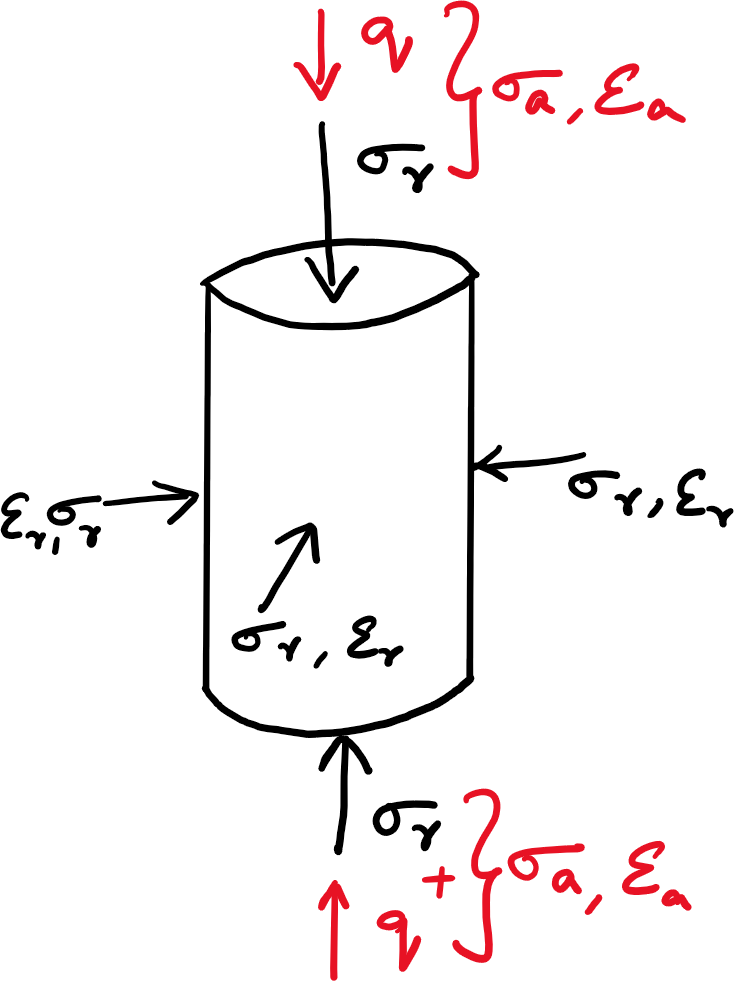
\includegraphics[width=0.9\textwidth]{figs/triaxial.png}
	\end{figure}
\end{minipage}	
\end{frame}

%----------------------------------------------------------------------------------------
\begin{frame}
\frametitle{Critical State Hypothesis: I}
Roscoe, Schofield \& Worth (1958): \textbf{At shear-failure, soil exists at a unique state}
\mode<beamer>{
	\begin{itemize}
		\item $d\varepsilon_q >> 0$ unlimited shear strain potential.
		\item $dp^\prime = dq = d\varepsilon_p = 0$ no change in $p^\prime, q, \varepsilon_p$.
		\item Critical state stress ratio: $\eta = q / p^\prime = const = M$ at failure $q = M p^\prime$.
	\end{itemize}
}
\mode<handout>{
	\vspace{3cm}
}
\begin{figure}
	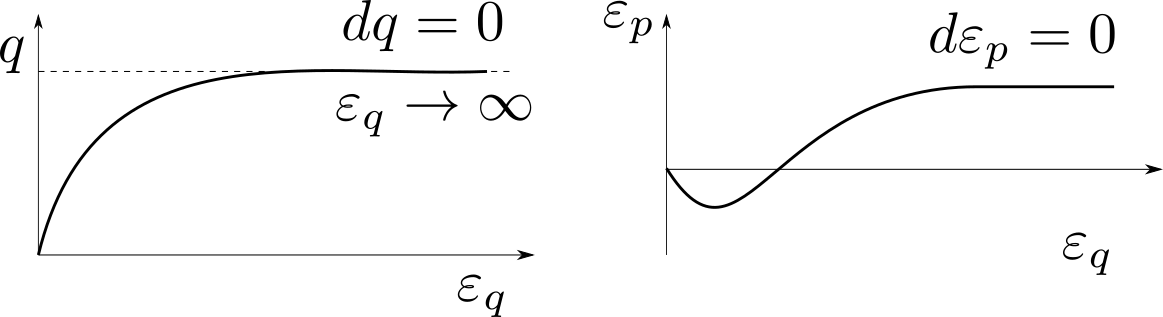
\includegraphics[width=0.9\textwidth]{figs/critical-state.png}
\end{figure}
\end{frame}
\note{Soil is sheared to a point where stresses are stationary $(dq = dp^\prime = 0)$ with no futher change in volume $(d\varepsilon_p = 0)$, unlimited shear strains $(d\varepsilon_q >> 0)$ and $q/p^\prime$ has a fixed value: \textbf{critical state}.

$M$ can be related to $phi^\prime$: $M = \frac{6\sin\phi^\prime}{3 - \sin\phi^\prime}$.
}


%----------------------------------------------------------------------------------------
\begin{frame}
\frametitle{Critical State Hypothesis: II}
\textbf{Critical state is a function of $q, p^\prime, v$. }
\begin{figure}
	\includegraphics[width=0.42\textwidth]{figs/critical-state-3d.png}
	\caption*{The CSL ($p^\prime, v, q$) space is given by the intersection of two planes: $q = Mp^\prime$ and a cruved vertical plane $v = \Gamma - \lambda \ln p^\prime$}
\end{figure}
\end{frame}

\note{Critical state curve connecting critical state points:
\begin{itemize}
	\item Crticial state line
	\item Defined in 3D but we'll look at projections into $q - p^\prime$ and $v - p^\prime$ space
\end{itemize}
}


%----------------------------------------------------------------------------------------
\begin{frame}
\frametitle{Critical State Hypothesis: II}
\textbf{Critical state is a function of $q, p^\prime, v$. }
\begin{figure}
	\includegraphics[width=\textwidth]{figs/critical-state-2d.png}
	\caption*{The CSL in (a) ($p^\prime, q$) plot and (b) ($p^\prime, v$) plot (isotropic normal compression line is shown in dashed)}
\end{figure}
\end{frame}

%----------------------------------------------------------------------------------------
\begin{frame}
\frametitle{Critical State Hypothesis: II}
\textbf{Critical state is a function of $q, p^\prime, v$. }
\begin{figure}
	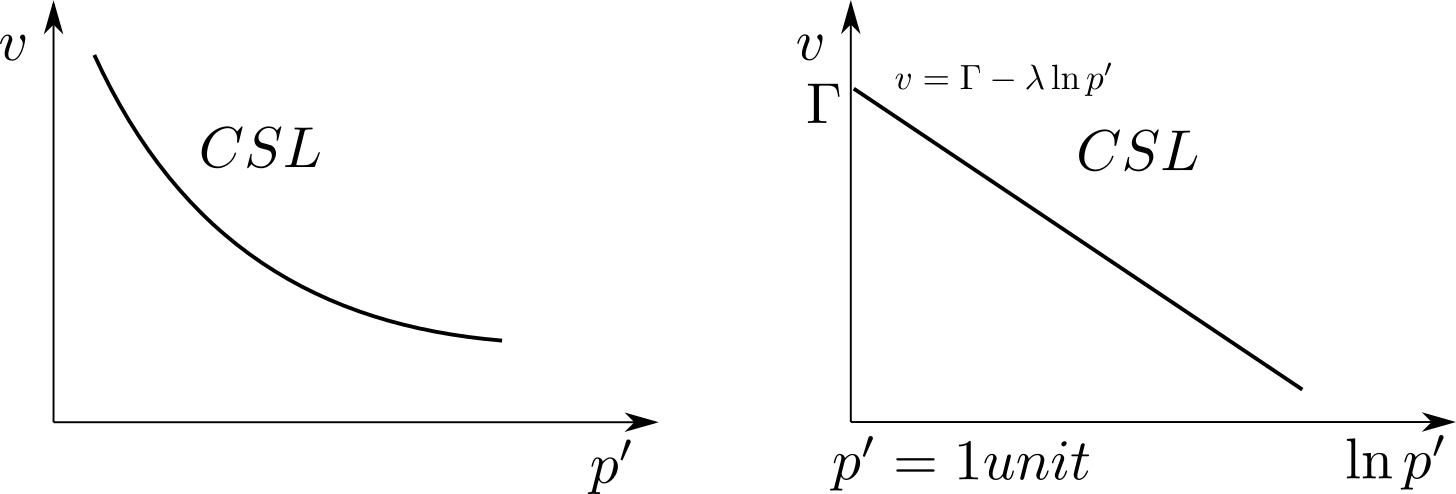
\includegraphics[width=\textwidth]{figs/v-lnp.png}
\end{figure}
\end{frame}

%----------------------------------------------------------------------------------------
\begin{frame}
\frametitle{Critical State Hypothesis: II}
\textbf{Critical state is a function of $q, p^\prime, v$. }
\begin{figure}
	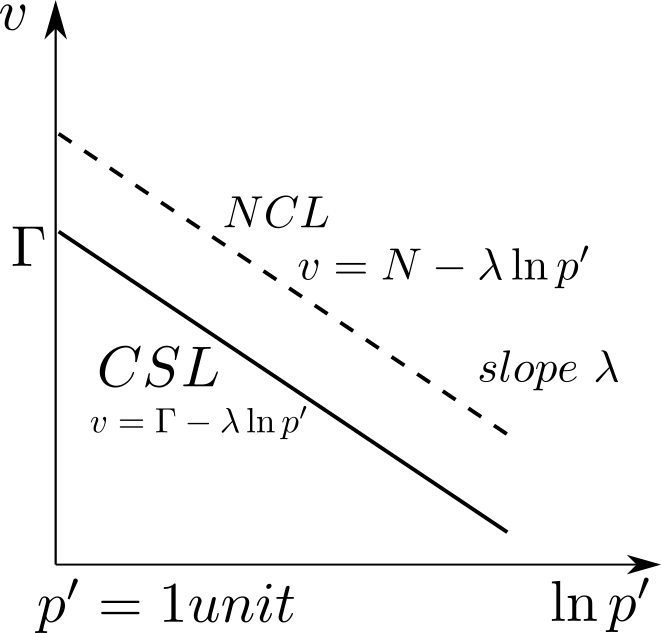
\includegraphics[width=0.6\textwidth]{figs/csl-ncl.png}
\end{figure}
\end{frame}

\note{
	Isotropic virgin compression line (VCL) $\eta = 0$. NCL is parallel to CSL. VCL is $\eta = 0$, while CSL $\eta = M$. Oedometer falls between VCL and CSL at a constant $\eta$: $0 < \eta < M$.
}


%----------------------------------------------------------------------------------------
\begin{frame}
\frametitle{Critical State Hypothesis: II}
\textbf{Critical state is a function of $q, p^\prime, v$. }
\begin{figure}
	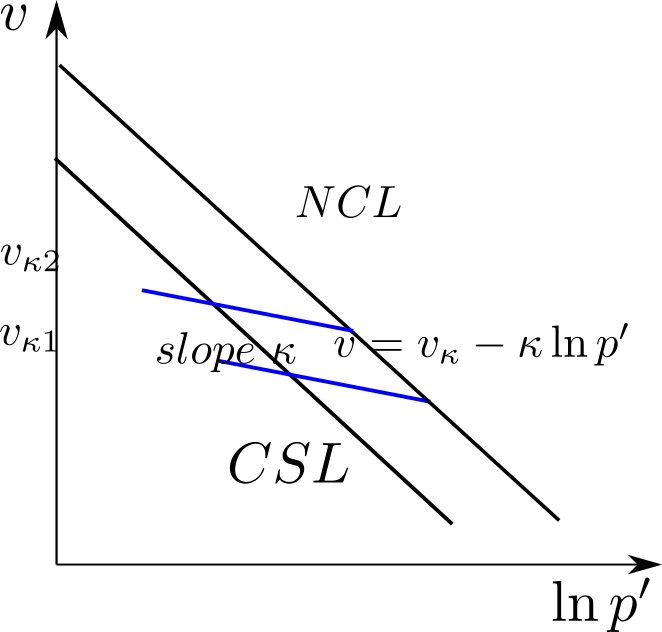
\includegraphics[width=0.65\textwidth]{figs/kappa.png}
\end{figure}
\end{frame}

\note{$v_\kappa$ depends on which $\kappa$ line you are on. $\kappa \ne c_r$ and $\lambda \ne C_c$}


%----------------------------------------------------------------------------------------
\begin{frame}
\frametitle{Stress paths $\sigma_3^\prime / \sigma_1^\prime = K_c = const$}
\begin{figure}
	\includegraphics[width=0.54\textwidth]{figs/stress-paths-kc.png}
\end{figure}
\end{frame}

%----------------------------------------------------------------------------------------
\begin{frame}
\frametitle{Clay behavior}
\begin{figure}
	\includegraphics[width=0.7\textwidth]{figs/clay-behavior.png}
\end{figure}
\end{frame}

%----------------------------------------------------------------------------------------
\begin{frame}
\frametitle{Critical state boundary surface}
\begin{figure}
	\includegraphics[width=0.45\textwidth]{figs/yieldsurface-3d.png}
\end{figure}
\end{frame}

%----------------------------------------------------------------------------------------
\begin{frame}
\frametitle{Summary of critical state behavior}
\mode<beamer>{
	\begin{itemize}
		\item Can only traverse NCL in one direction
		\item Can traverse RCL ($\kappa$-line) in both directions
		\item To move from one $\kappa$-line to another must move along NCL. Hence, plastic volumetric strains must occur.
		\item Critical state line is \textbf{NOT} a yield surface. It's where it's going but a lot of plastic straining is needed to get there. (if $CSL = F = 0$) then with associative flow rule $d\varepsilon_p^p \ne0$ at critical state. Real $F$ is horizontal at critical state.
	\end{itemize}
}
\mode<handout>{
	\vspace{3cm}
}
\end{frame}
\end{document}
